\section{Question 4}

\subsection{The Question}

\begin{flushleft}

 Use MDS to create a JPEG of the blogs similar to slide 29.  
How many iterations were required?

\end{flushleft}
\subsection{The Answer}


The Python function used to produce the MDS plot is provided in the book \cite{PCI}. The algorithm required 353 iterations to converge. The terminal output it attached.

\lstset{
    language=Python,
    label=code:q1,
    caption={Python script to produce dendrograms}
}
\lstinputlisting{../q4/q4.py}


\begin{figure}
\centering
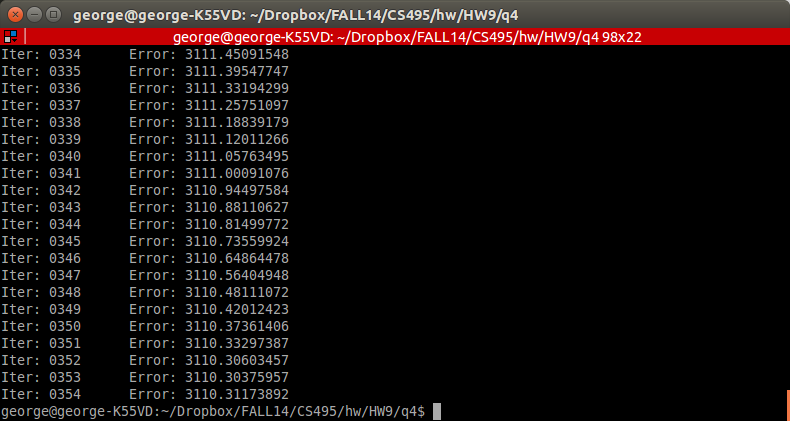
\includegraphics[width=\textwidth]{../q4/mds.png}
\caption{Terminal output from Multi-Dimensional Scaling}
\end{figure}

\begin{figure}
\centering
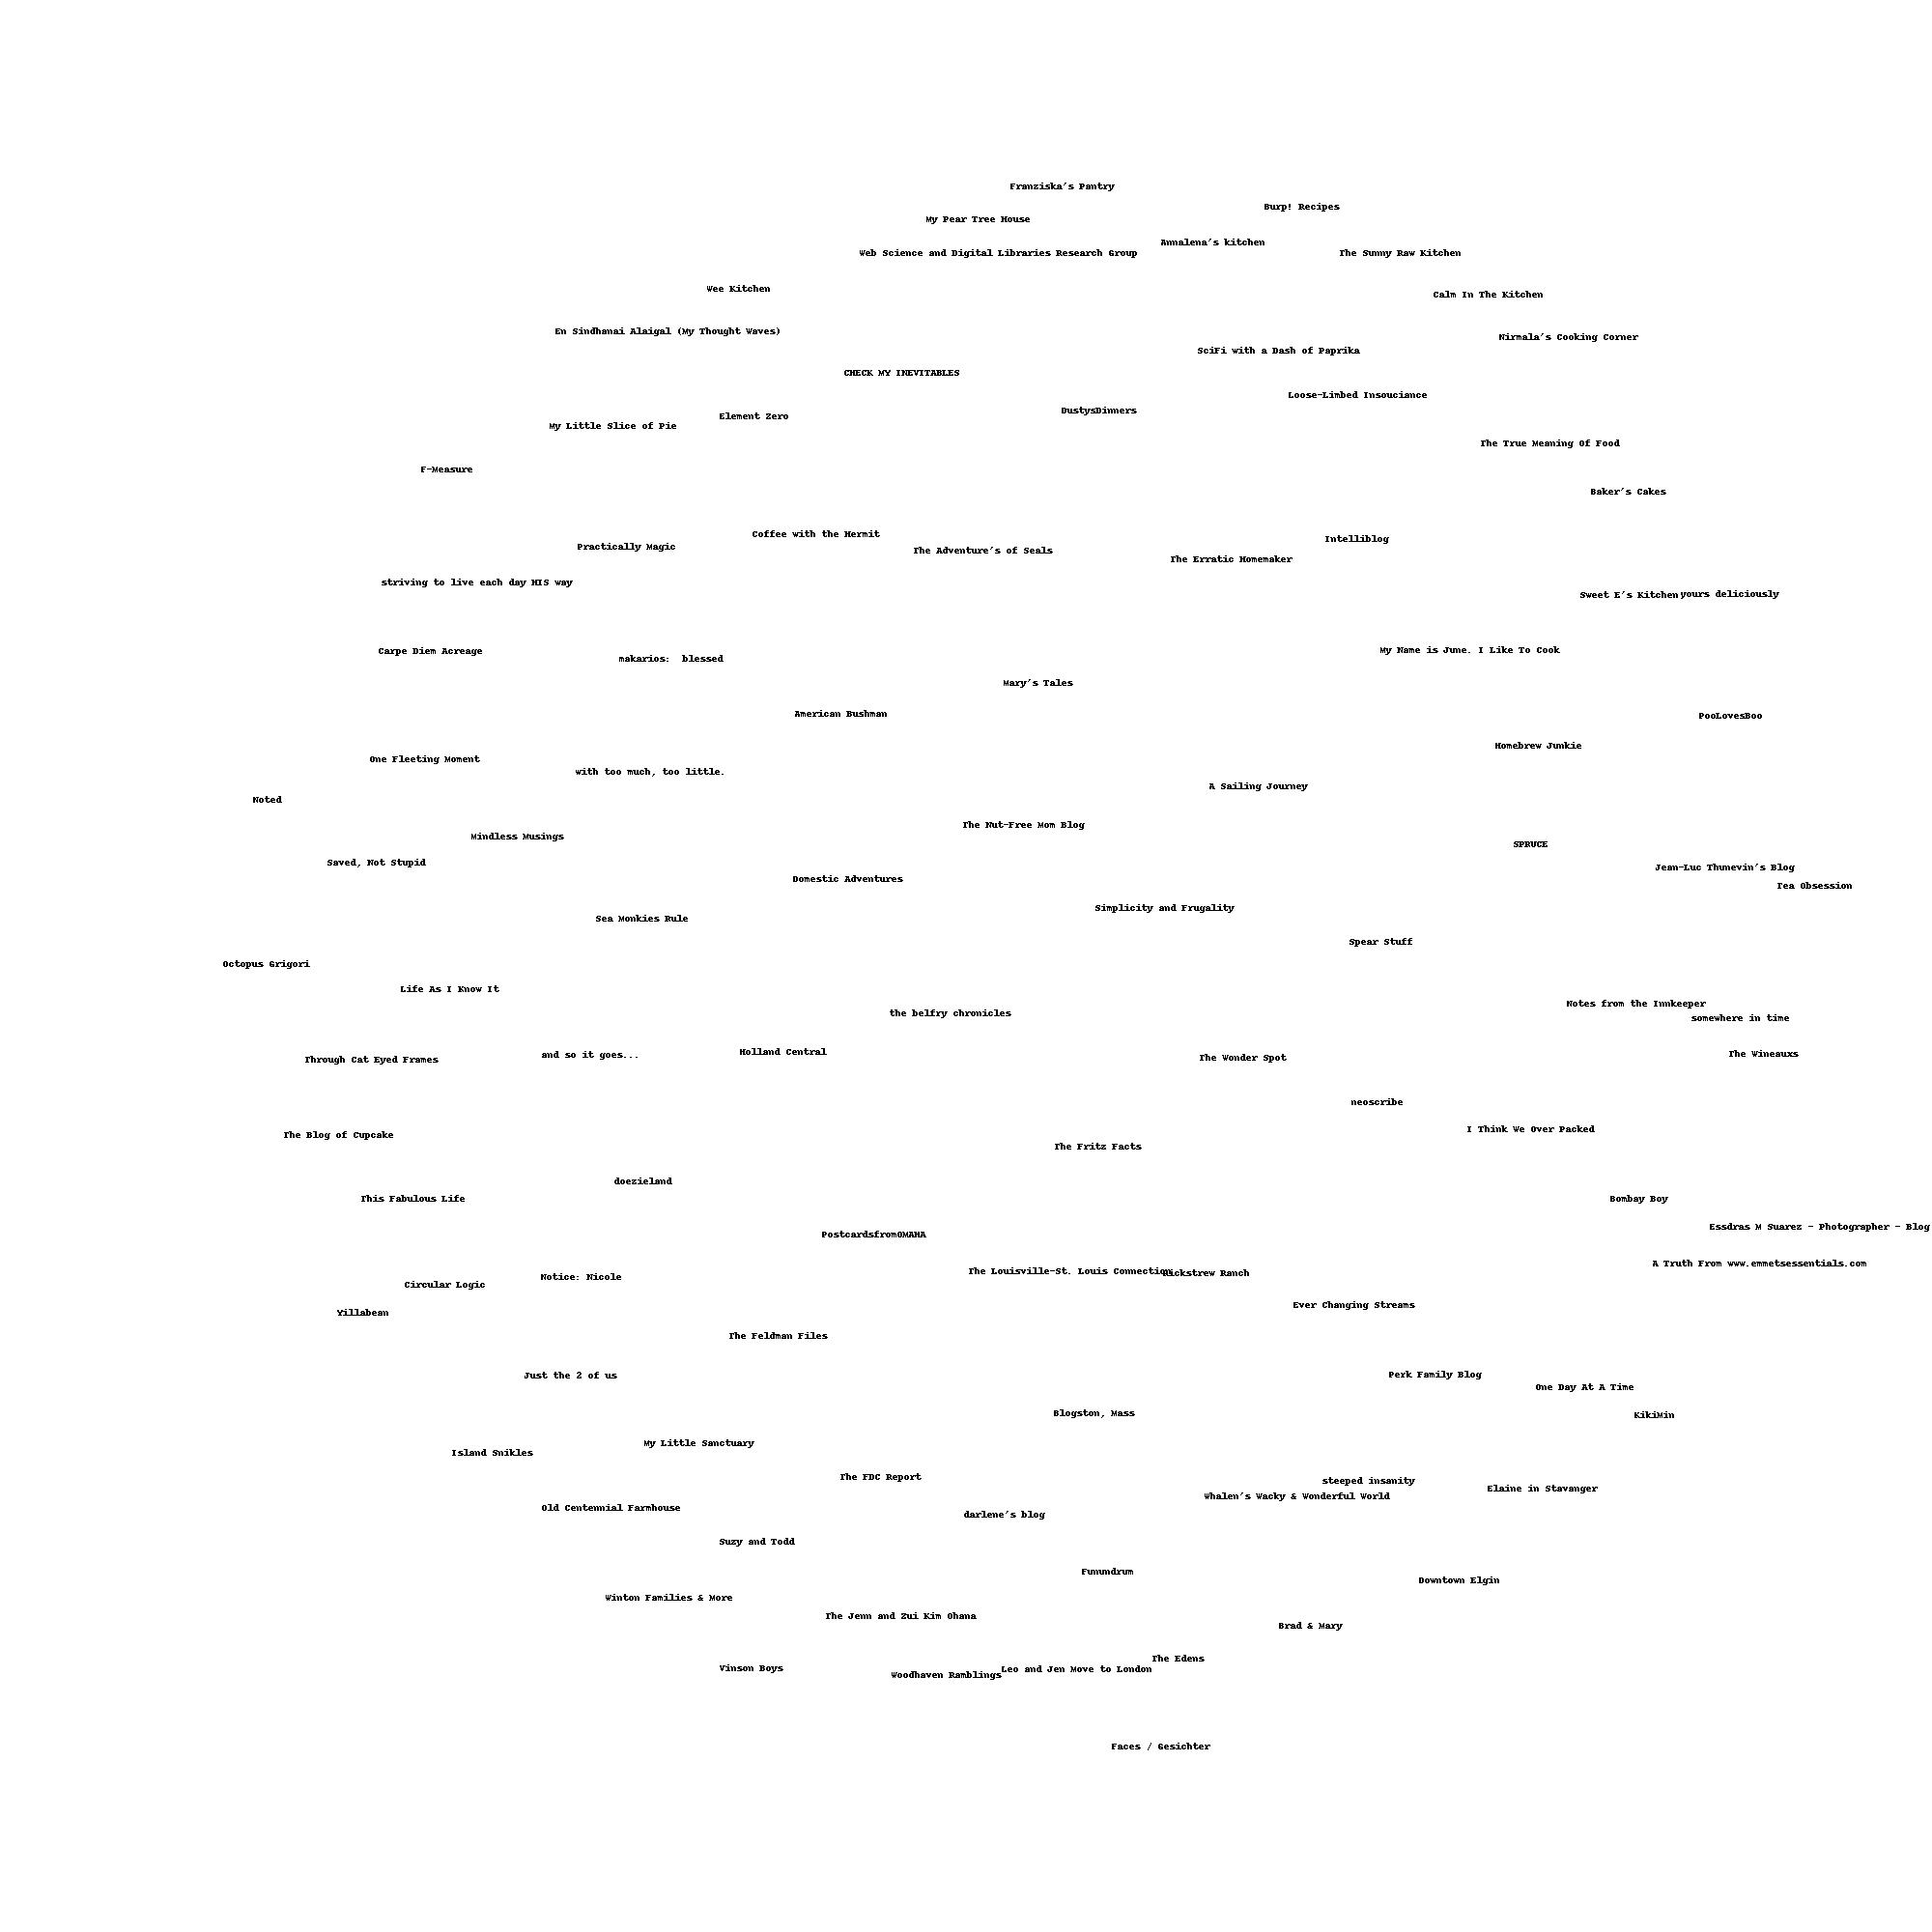
\includegraphics[width=\textwidth]{../q4/blogs2d}
\caption{Multi-Dimensional Scaling of the blogs}
\end{figure}




